\documentclass{article}
\iffalse
This file is protected by Copyright. Please refer to the COPYRIGHT file
distributed with this source distribution.

This file is part of OpenCPI <http://www.opencpi.org>

OpenCPI is free software: you can redistribute it and/or modify it under the
terms of the GNU Lesser General Public License as published by the Free Software
Foundation, either version 3 of the License, or (at your option) any later
version.

OpenCPI is distributed in the hope that it will be useful, but WITHOUT ANY
WARRANTY; without even the implied warranty of MERCHANTABILITY or FITNESS FOR A
PARTICULAR PURPOSE. See the GNU Lesser General Public License for more details.

You should have received a copy of the GNU Lesser General Public License along
with this program. If not, see <http://www.gnu.org/licenses/>.
\fi

\author{} % Force author to be blank
%----------------------------------------------------------------------------------------
% Paper size, orientation and margins
%----------------------------------------------------------------------------------------
\usepackage{geometry}
\geometry{
	letterpaper,			% paper type
	portrait,				% text direction
	left=.75in,				% left margin
	top=.75in,				% top margin
	right=.75in,			% right margin
	bottom=.75in			% bottom margin
 }
%----------------------------------------------------------------------------------------
% Header/Footer
%----------------------------------------------------------------------------------------
\usepackage{fancyhdr} \pagestyle{fancy} % required for fancy headers
\renewcommand{\headrulewidth}{0.5pt}
\renewcommand{\footrulewidth}{0.5pt}
\newcommand{\terminaloutput}[1]{\texttt{#1}}
\rhead{\small{ANGRYVIPER Team}}
%----------------------------------------------------------------------------------------
% Appendix packages
%----------------------------------------------------------------------------------------
\usepackage[toc,page]{appendix}
%----------------------------------------------------------------------------------------
% Defined Commands & Renamed Commands
%----------------------------------------------------------------------------------------
\renewcommand{\contentsname}{Table of Contents}
\renewcommand{\listfigurename}{List of Figures}
\renewcommand{\listtablename}{List of Tables}
\newcommand{\todo}[1]{\textcolor{red}{TODO: #1}\PackageWarning{TODO:}{#1}} % To do notes
\newcommand{\code}[1]{\texttt{#1}} % For inline code snippet or command line
%----------------------------------------------------------------------------------------
% Various pacakges
%----------------------------------------------------------------------------------------
\usepackage{hyperref} % for linking urls and lists
\usepackage{graphicx} % for including pictures by file
\usepackage{listings} % for coding language styles
\usepackage{rotating} % for sideways table
\usepackage{pifont}   % for sideways table
\usepackage{pdflscape} % for landscape view
\usepackage{scrextend}
%----------------------------------------------------------------------------------------
% Table packages
%----------------------------------------------------------------------------------------
\usepackage{longtable} % for long possibly multi-page tables
\usepackage{tabularx} % c=center,l=left,r=right,X=fill
\usepackage{float}
\floatstyle{plaintop}
\usepackage[tableposition=top]{caption}
\newcolumntype{P}[1]{>{\centering\arraybackslash}p{#1}}
\newcolumntype{M}[1]{>{\centering\arraybackslash}m{#1}}
%----------------------------------------------------------------------------------------
% Block Diagram / FSM Drawings
%----------------------------------------------------------------------------------------
\usepackage{tikz}
\usetikzlibrary{shapes,arrows,fit,positioning}
\usetikzlibrary{automata} % used for the fsm
\usetikzlibrary{calc} % For duplicating clients
\usepgfmodule{oo} % To define a client box
%----------------------------------------------------------------------------------------
% Colors Used
%----------------------------------------------------------------------------------------
\usepackage{colortbl}
\definecolor{blue}{rgb}{.7,.8,.9}
\definecolor{ceruleanblue}{rgb}{0.16, 0.32, 0.75}
\definecolor{drkgreen}{rgb}{0,0.6,0}
\definecolor{deepmagenta}{rgb}{0.8, 0.0, 0.8}
\definecolor{cyan}{rgb}{0.0,0.6,0.6}
\definecolor{maroon}{rgb}{0.5,0,0}
\usepackage{multirow}
%----------------------------------------------------------------------------------------
% Update the docTitle and docVersion per document
%----------------------------------------------------------------------------------------
\def\docTitle{Component Data Sheet}
\def\docVersion{1.4}
%----------------------------------------------------------------------------------------
\date{Version \docVersion} % Force date to be blank and override date with version
\title{\docTitle}
\lhead{\small{\docTitle}}

% find and replace: dev signal, devsignal -> \devsignal{}
\def\devsignal{devsignal}
% find and replace: Dev Signal, Dev signal, dev Signal, DevSignal -> \DevSignal{}
\def\DevSignal{DevSignal}

\def\comp{ad9361\_spi}
\edef\ecomp{ad9361_spi}
\def\Comp{AD9361 SPI}
\graphicspath{ {figures/} }

\begin{document}

\section*{Summary - \Comp}
\begin{tabular}{|c|M{13.5cm}|}
	\hline
	\rowcolor{blue}
	                  &                  \\
	\hline
	Name              & \comp            \\
	\hline
	Worker Type       & Device           \\
	\hline
	Version           & v\docVersion{}   \\
	\hline
	Release Date      & October 2018         \\
	\hline
	Component Library & ocpi.assets.devices     \\
	\hline
	Workers           & \comp.hdl        \\
	\hline
	Tested Platforms  & Zedboard (ISE), Zedboard (Vivado), ML605 (FMC LPC slot) \\
	\hline
\end{tabular}
\section*{Functionality}
	The \Comp{} subdevice worker implements a SPI state machine for communication with the AD9361 IC\cite{ad9361}.
\section*{Worker Implementation Details}
\subsection*{\comp.hdl}
The \comp{}.hdl subdevice worker is intend for use in platforms/cards where a SPI bus exists which addresses only the AD9361. SPI read/writes are actuated by the \verb+rprops+ rawprop port. A \devsignal{} is also sent in which can force the AD9361 RESETB pin, which is active-low, to logic 0.
\section*{Block Diagrams}
\subsection*{Top level}
\makeatletter
\newcommand{\gettikzxy}[3]{%
  \tikz@scan@one@point\pgfutil@firstofone#1\relax
  \edef#2{\the\pgf@x}%
  \edef#3{\the\pgf@y}%
}
\makeatother
\pgfooclass{clientbox}{ % This is the class clientbox
    \method clientbox() { % The clientbox
    }
    \method apply(#1,#2,#3,#4) { % Causes the clientbox to be shown at coordinate (#1,#2) and named #3
        \node[rectangle,draw=white,fill=white] at (#1,#2) (#3) {#4};
    }
}
\pgfoonew \myclient=new clientbox()
\begin{center}
  \begin{tikzpicture}[% List of styles applied to all, to override specify on a case-by-case
      every node/.style={
        align=center,      % use this so that the "\\" for line break works
        minimum size=1cm,  % creates space above and below text in rectangle
      },
      every edge/.style={draw,thick}
    ]
    \node[rectangle,ultra thick,draw=black,fill=blue,minimum size=2cm,minimum width=12.5cm](R1){\Comp};
    \node[rectangle,draw=white,fill=white](R4)[above= of R1]{ };
    \gettikzxy{(R4)}{\rx}{\ry}
    \node[rectangle,draw=white,fill=white] at (\rx-50,\ry) (C1) {Non-parameter Properties:\\ \verb+lastAddr+ \\ \verb+lastData+ \\ \verb+resetting+};
    \path[<-]($(R1.north) + (-50 pt,0)$) edge [] node [] {} (C1);
    \myclient.apply(\rx + 160,\ry,C1, ``rprops'' \\ rawprop port \\ sent from \\ ad9361\_config.hdl);
    \path[<-]($(R1.north) + (160 pt,0)$) edge [] node [] {} (C1);
     \myclient.apply(\rx + 70,\ry,C1, ``dev\_force\_reset'' \\ \devsignal{} port \\ sent from \\ ad9361\_config.hdl);
    \path[<-]($(R1.north) + (70 pt,0)$) edge [] node [] {} (C1);
     \myclient.apply(\rx ,\ry - 150,C1, Signals:\\ SPI\_DI, SPI\_CLK, SPI\_ENB, SPI\_DO, RESETB );
    \path[<->]($(R1.south) + (0, 0 pt)$) edge [] node [] {} (C1);
  \end{tikzpicture}
\end{center}

\section*{Source Dependencies}
\subsection*{\comp.hdl}
\begin{itemize}
	\item assets/hdl/devices/\comp{}.hdl/comp{}.vhd
	\item assets/hdl/devices/\comp{}.hdl/signals.vhd
	\item assets/hdl/primitives/util/spi.vhd
	\item assets/hdl/primitives/util/util\_pkg.vhd
\end{itemize}
\begin{landscape}

	\section*{Component Spec Properties}
	\begin{scriptsize}
		\begin{tabular}{|p{3.75cm}|p{1.25cm}|p{2cm}|p{2.75cm}|p{1.5cm}|p{1.5cm}|p{1cm}|p{5.25cm}|}
			\hline
			\rowcolor{blue}
			Name               & Type & SequenceLength & ArrayDimensions & Accessibility      & Valid Range & Default & Usage                                                                               \\
			\hline
			\verb+CP_CLK_FREQ_HZ_p+ & Float & -              & -               & Parameter  & Standard    & 100e6   & Value will determine assumed frequency of the Control Plane (CP) clock. This value is used to calculate the dividor for the SPI clock              \\
			\hline
			\verb+SPI_CLK_FREQ_HZ_p+ & Bool & -              & -               & Parameter & Standard    & 6.25e6  & - \\
			\hline
			\verb+lastAddr+ & UShort & -              & -               & Volatile & Standard    & - & - \\
			\hline
			\verb+lastAddr+ & UChar & -              & -               & Volatile & Standard    & - & - \\
			\hline
			\verb+lastAddr+ & Bool & -              & -               & Volatile & Standard    & - & - \\
			\hline
		\end{tabular}
	\end{scriptsize}

	\section*{Worker Properties}
	\subsection*{\comp.hdl}
	\begin{scriptsize}
		\begin{tabular}{|p{2cm}|p{2cm}|p{1cm}|p{2cm}|p{2cm}|p{2cm}|p{2cm}|p{1cm}|p{4.58cm}|}
			\hline
			\rowcolor{blue}
			Scope        & Name                 & Type & SequenceLength & ArrayDimensions & Accessibility & Valid Range        & Default & Usage                                                                                                                  \\
			\hline
			- & - & - & - & - & - & - & - & - \\
			\hline
		\end{tabular}
	\end{scriptsize}

	\section*{Component Ports}
	\begin{scriptsize}
		\begin{tabular}{|p{2cm}|p{1.5cm}|p{4cm}|p{1.5cm}|p{1.5cm}|p{9.38cm}|}
			\hline
			\rowcolor{blue}
			Name & Producer & Protocol           & Optional & Advanced & Usage                  \\
			\hline
			-  & -     & - & -     & -        & - \\
			\hline
		\end{tabular}
	\end{scriptsize}
	\section*{Worker Interfaces}
	\subsection*{\comp.hdl}
	\begin{scriptsize}
		\begin{tabular}{|p{2cm}|p{1.5cm}|p{1.5cm}|p{15.74cm}|}
			\hline
			\rowcolor{blue}
			Type            & Name & Optional & Usage                  \\
			\hline
			RawProp & rprops  & True & - \\
			\hline
		\end{tabular}
	\end{scriptsize} \\
	\begin{scriptsize}
		\begin{tabular}{|p{1.5cm}|p{2.4cm}|p{1.05cm}|p{1.25cm}|p{1.2cm}|p{2cm}|p{1.4cm}|p{0.9cm}|p{6.88cm}|}
			\hline
			\rowcolor{blue}
			Type                       & Name                            & Count & Optional & Master                & Signal                & Direction                  & Width                    & Description                                                                                                                  \\
			\hline
			DevSignal & dev\_force\_spi\_reset & 1 & False & False & force\_reset & Output & 1 & Used to force AD9361 RESETB pin, which is active-low, to logic 0. \\
			\hline
		\end{tabular}
	\end{scriptsize}
\end{landscape}

\section*{Control Timing and Signals}
The \Comp{}.hdl device worker operates entirely in the control plane clock domain. All SPI data and SPI clock signals are generated in the control plane clock domain. Note that SPI clock can only be a divided version of the control plane clock.

\section*{Worker Configuration Parameters}
\subsubsection*{\comp.hdl}
\input{../../\ecomp.hdl/configurations.inc}
\section*{Performance and Resource Utilization}
\subsubsection*{\comp.hdl}
Fmax refers to the maximum allowable clock rate for any registered signal paths within a given clock domain for an FPGA design. Fmax in the table below is specific only to this worker and represents the maximum possible Fmax for any OpenCPI bitstream built with this worker included. Note that the Fmax value for a given clock domain for the final bitstream is often worse than the Fmax specific to this worker, even if this worker is the only one included in the bitstream.

%\input{../../\ecomp.hdl/utilization.inc}
\input{utilization_custom.inc}

\footnotetext[1]{\label{abc}These measurements were the result of a Vivado timing analysis which was different from the Vivado analysis performed by default for OpenCPI worker builds. For more info see Appendix \ref{appendix}}

\section*{Test and Verification}
The test outlined in \cite{dac_comp_datasheet} includes validation of a subset of this worker's functionality.

\begin{thebibliography}{1}

\bibitem{ad9361} AD9361 Datasheet and Product Info \\
\url{http://www.analog.com/en/products/rf-microwave/integrated-transceivers-transmitters-receivers/wideband-transceivers-ic/ad9361.html}
\bibitem{adi_ug570} AD9361 Reference Manual UG-570\\
AD9361\_Reference\_Manual\_UG-570.pdf
 \bibitem{dac_comp_datasheet} AD9361 DAC Component Data Sheet \\
 \url{https://opencpi.github.io/assets/AD9361_DAC.pdf}

\end{thebibliography}
\pagebreak
\section{Appendix - Vivado Timing Analysis} \label{appendix}

The Vivado timing report that OpenCPI runs for device workers may erroneously report a max delay for a clocking path which should have been ignored. Custom Vivado tcl commands had to be run for this device worker to extract pertinent information from Vivado timing analysis. After building the worker, the following commands were run from the base project directory (after the Vivado settings64.sh was sourced):
\lstset{language=bash, backgroundcolor=\color{lightgray}, columns=flexible, breaklines=true, prebreak=\textbackslash, basicstyle=\ttfamily, showstringspaces=false,upquote=true, aboveskip=\baselineskip, belowskip=\baselineskip}
\begin{lstlisting}
cd hdl/devices/
vivado -mode tcl
\end{lstlisting}
Then the following commands were run inside the Vivado tcl terminal for the parameter property set:
\begin{itemize}
	\item \verb+CP_CLK_FREQ_HZ_p+=100e6
	\item \verb+SPI_CLK_FREQ_HZp+=6.25e6
\end{itemize}
\begin{lstlisting}
open_project ad9361_spi.hdl/target-zynq/ad9361_spi_rv.xpr
synth_design -part xc7z020clg484-1 -top ad9361_spi_rv -mode out_of_context
create_clock -name clk1 -period 0.001 [get_nets {ctl_in[Clk]}]
report_timing -delay_type min_max -sort_by slack -input_pins -group clk1
\end{lstlisting}
The Fmax for the control plane clock for this worker is computed as the maximum magnitude slack with a control plane clock of 1 ps plus 2 times the assumed 1 ps control plane clock period (4.244 ns + 0.002 ns = 4.244 ns, 1/4.244 ns = 235.52 MHz).
Then the following commands were run inside the Vivado tcl terminal for the parameter property set:
\begin{itemize}
	\item \verb+CP_CLK_FREQ_HZ_p+=125e6
	\item \verb+SPI_CLK_FREQ_HZp+=6.25e6
\end{itemize}
\begin{lstlisting}
open_project ad9361_spi.hdl/target-1-zynq/ad9361_spi_rv.xpr
synth_design -part xc7z020clg484-1 -top ad9361_spi_rv_c1 -mode out_of_context
create_clock -name clk1 -period 0.001 [get_nets {ctl_in[Clk]}]
report_timing -delay_type min_max -sort_by slack -input_pins -group clk1
\end{lstlisting}
The Fmax for the control plane clock for this worker is computed as the maximum magnitude slack with a control plane clock of 1 ps plus 2 times the assumed 1 ps control plane clock period (3.169 ns + 0.002 ns = 3.171 ns, 1/3.171 ns = 315.36 MHz).

\end{document}
